\section{Verification by finite element analysis}
\subsection{Simulation Setup and Case Study}

Động cơ nam châm vĩnh cửu dọc trục (AFPM) với cấu trúc 30 rãnh và 20 cực, sử dụng dây quấn tập trung (concentrated winding) được lựa chọn để kiểm chứng tính chính xác của phương pháp 3D-MBGRN. Các thông số hình học, thông số định mức và đặc tính vật liệu chi tiết của mô hình được liệt kê trong Bảng \ref{afpm_par}. Trong đó, nam châm vĩnh cửu sử dụng vật liệu NdFe30 và lõi sắt được chế tạo từ thép 1008.

\begin{table}[ht]
\centering
\caption{Main parameter of the AFPM}
\begin{tabular}{lcc}
\hline
\textbf{Parameters} && \textbf{Value}\\
Rated power         && 3.0 $kW$      \\
Rated voltage       && 400 $V$       \\ 
Rated current       && 10 $A$        \\ 
Rated torque        && 10 $Nm$        \\
Rated speed         && 3000 $rpm$     \\
Slot number         && 30  \\ 
Pole number         && 15 \\ 
Stator outer diameter && 150 $mm$ \\ 
Stator inner diameter && 70 $mm$ \\ 
Stator length       && 25 $mm$ \\
Rotor outer diameter && 150 $mm$ \\ 
Rotor inner diameter && 70 $mm$ \\ 
Rotor length && 6 $mm$ \\ 
Air gap length         && 1.5 $mm$ \\ 
Magnet grade           && NdFe30 \\
Lamination grade       && steel 1008 \\
\hline
\end{tabular}
\label{afpm_par}
\end{table}

Để đơn giản hóa và tăng tốc quá trình tính toán, hệ số tuần hoàn $k_s = 5$ và điều kiện biên chu kỳ được áp dụng cho cả hai phương pháp 3D-MRN và FEM, tương ứng với việc sử dụng $1/5$ mô hình theo phương $\theta$. Điều kiện biên Dirichlet được áp dụng trên ranh giới trong và ngoài của stator và rotor trong cả hai phương pháp.

Mật độ lưới của cả hai phương pháp cũng được tinh chỉnh để đạt độ chính xác cao nhất. Đối với 3D-MRN, tại các khu vực xuất hiện biến dạng hình học đáng kể do quá trình rời rạc hóa, mật độ nút lưới được tăng cường nhằm mô tả trung thực sự phân bố từ trường. Trong khi đó, các khu vực tương ứng trong mô hình FEM được kiểm soát thông qua việc thiết lập kích thước phần tử tối đa (maximum element size). Đặc biệt, số lượng lớp phần tử trong miền khe hở không khí của cả hai mô hình được cài đặt không ít hơn 4 lớp nhằm đảm bảo tính chính xác khi trích xuất các thành phần mật độ từ thông phục vụ tính toán ứng suất Maxwell.

\begin{figure}
    \centering
    \includegraphics[width=0.5\textwidth]{figure/mesh.png}
    \caption{Miền tính toán rút gọn và cấu hình lưới trên FEM và 3D-MRN}
    \label{fig4}
\end{figure}

Ngoài ra, các cấu hình lưới sử dụng trong nghiên cứu này đều đã trải qua quá trình kiểm tra tính hội tụ để đảm bảo sự cân bằng giữa độ chính xác và chi phí tính toán. Các kết quả trình bày dưới đây được thực hiện với mật độ lưới đã đạt tới ngưỡng hội tụ, nghĩa là kể từ mật độ lưới này trở đi, nếu tiếp tục tinh chỉnh lưới dày hơn thì sai số NRMSE của kết quả dạng sóng tính toán không vượt quá 5\%.

Nhằm đảm bảo tính tương đồng khi so sánh kết quả, số lượng bước tính toán trong một chu kỳ mô phỏng của cả hai phương pháp được thiết lập bằng nhau và bằng $n$, với $n = 30$. Trong nghiên cứu này, đặc tính mô-men răng (cogging torque) được lựa chọn làm đại lượng kiểm chứng chính. Một chu kỳ biến thiên của mô-men răng theo góc cơ học được xác định bởi biểu thức:
\begin{equation}
    \theta_{cog} = \frac{2\pi}{\text{LCM}(Q, 2p)}
\end{equation}
Trong đó, $Q$ là số rãnh stator và $2p$ là số cực từ. Do mô hình 3D-MRN thực hiện tính toán dựa trên các bước quay rời rạc, để thu được $n$ điểm dữ liệu trên toàn bộ chu kỳ cogging, bước góc quay $\Delta\theta$ giữa hai lần giải liên tiếp được xác định như sau:
\begin{equation}
    \Delta\theta = \frac{\theta_{cog}}{n}
\end{equation}
Việc lựa chọn $n=30$ bước tính cho một chu kỳ $\theta_{cog}$ đảm bảo độ phân giải đủ cao để quan sát các đỉnh dao động của mô-men điện từ và đánh giá sai số giữa mô hình mạng điện trở từ và phương pháp phần tử hữu hạn.

\subsection{No Load Verification}
Theo \cite{10599821}, việc xác minh trạng thái không tải là một bước nền tảng không thể thiếu và có ý nghĩa quyết định trong bài toán mô hình hóa điện từ của máy điện. Việc thực hiện mô phỏng trong điều kiện hở mạch giúp cô lập hoàn toàn hệ thống khỏi từ trường phản ứng phần ứng phức tạp do dòng điện dây quấn stator gây ra, từ đó cho phép người thiết kế quan sát và kiểm chứng một cách thuần túy quy luật phân bố từ trường cơ bản được thiết lập bởi hệ thống nam châm vĩnh cửu. Bên cạnh đó, giai đoạn này còn cung cấp một chuẩn mực nghiêm ngặt để đánh giá chất lượng của quá trình rời rạc hóa lưới phi tham số. Nó đóng vai trò then chốt trong việc xác minh xem bộ giải lặp điểm bất động phi tuyến kết hợp với kỹ thuật thư giãn vật liệu thích nghi có khả năng phản ánh chính xác hiện tượng bão hòa từ tính cục bộ bên trong lõi sắt từ dưới tác động kích từ đơn lẻ của nam châm hay không. Do đó, một kết quả tính toán trường không tải chính xác sẽ thiết lập một nền tảng toán học vững chắc trước khi mở rộng sang các phân tích động lực học có tải phức tạp hơn.

Để chứng minh tính đúng đắn của phương pháp mạng từ trở 3 chiều đề xuất (3D-MRN), các kết quả mô phỏng ở trạng thái không tải thu được từ bộ giải được đặt trong sự đối chiếu trực tiếp với kết quả từ phương pháp phần tử hữu hạn (3D-FEM). Trước hết, phân bố mật độ từ thông tổng thể trên toàn bộ cấu trúc máy điện được mô tả trực quan thông qua bản đồ từ trường (B-map) tại Hình~\ref{bmap_no_load} qua 3 góc nhìn phân tích bao gồm (a) phối cảnh (isometric view), (b) mặt cắt ngang giữa khe hở không khí (mid-airgap cross-sectional view) với một probe line để phục vụ việc thu thập các kết quả định lượng của từ trường cục bộ, và (c) mặt đáy (bottom surface view). Kết quả thu được cho thấy một sự tương đồng rất cao về quy luật phân bố tổng thể giữa phương pháp 3D-MBGRN đề xuất và phương pháp 3D-FEM đối chứng. Hình \ref{bmap_no_load} cho thấy sự tương đồng về quy luật độ lớn của phân bố mật độ từ thông, mặc dù kết quả thu được từ 3D-MBGRN là một bản đồ rời rạc do sử dụng cấu trúc phần tử hình lục diện.

\begin{figure}[H]
    \centering
    \includegraphics[width=0.48\textwidth]{figure/bmap_no_load.png}
    \caption{Comparison of magnetic flux density distributions between FEM and the proposed 3D-MBGRN solver: (a) 3D isometric view, (b) cross-sectional view at the mid-airgap plane with the highlighted airgap probing path, and (c) bottom surface view.}
    \label{bmap_no_load}
\end{figure}

% Airgap flux density
Nhằm có một đánh giá khách quan về quy luật phân bố điện từ, các kết quả về từ thông khe hở không khí theo các phương bán kính $B_r$, tiếp tuyến $B_{\theta}$ và dọc trục $B_z$ được trích xuất tại một cung tròn nằm trong mặt phẳng giữa khe hở không khí, tại bán kính trung bình như trong hình \ref{bmap_no_load}.b. Kết quả về dạng sóng theo thời gian và phổ harmonic được đưa ra trong các hình \ref{airgap_flux_density_no_load} và \ref{airgap_flux_density_no_load_harmonic}:

\begin{figure}[H]
    \centering
    \includegraphics[width=0.45\textwidth]{figure/airgap_flux_density_no_load_waveform.png}
    \caption{Mật độ từ thông khe hở không khí theo các phương bán kính, tiếp tuyến và dọc trục}
    \label{airgap_flux_density_no_load}
\end{figure}

\begin{figure}[H]
    \centering
    \includegraphics[width=0.45\textwidth]{figure/airgap_flux_density_no_load_harmonics.png}
    \caption{Phổ sóng hài mật độ từ thông khe hở không khí}
    \label{airgap_flux_density_no_load_harmonic}
\end{figure}

Các kết quả thu được trong hình \ref{airgap_flux_density_no_load} cho thấy sự tương đồng khá rõ về pha, biên độ và dạng sóng giữa bộ giải 3D-MBGRN đề xuất và mô hình 3D-FEM đối chứng. Trong động cơ hướng trục, thành phần mật độ từ thông dọc trục ($B_z$) đóng vai trò chủ đạo, ghi nhận giá trị đỉnh $0.74\text{ T}$ ở 3D-MBGRN so với $0.73\text{ T}$ ở 3D-FEM (độ lệch tương đối khoảng $1.09\%$) và trị hiệu dụng RMS tương ứng đạt $0.62\text{ T}$ (độ lệch $0.58\%$). Thành phần tiếp tuyến ($B_\theta$) có biên độ đỉnh ghi nhận ở mức $0.25\text{ T}$ so với $0.23\text{ T}$ (độ lệch $8.12\%$), trong khi thành phần bán kính ($B_r$) có giá trị tương đối nhỏ.

Kết quả phân tích phổ sóng hài không gian trong hình \ref{airgap_flux_density_no_load_harmonic} cho thấy thành phần sóng hài bậc cơ bản (Harmonic Order \#1) của mật độ từ thông dọc trục $B_z$ đạt mức tương đồng cao giữa hai phương pháp, với giá trị $0.8432\text{ T}$ đối với 3D-MBGRN và $0.8437\text{ T}$ đối với 3D-FEM (độ lệch tương đối xấp xỉ $0.07\%$). Các thành phần sóng hài bậc cao như bậc 3 ($0.1906\text{ T}$ so với $0.1768\text{ T}$, độ lệch $7.78\%$) và bậc 5 ($0.0871\text{ T}$ so với $0.0621\text{ T}$) phản ánh ảnh hưởng của hiện tượng bão hòa từ tính phi tuyến trong lõi sắt thép 1008, cho thấy khả năng đáp ứng phù hợp của phương pháp mạng từ trở sinh lưới đề xuất.

% Flux linkage 
Trong số các đặc tính vận hành toàn cục của máy điện, từ thông liên kết ($\Psi$) đóng vai trò là một đại lượng cốt lõi, tạo nên mối liên kết điện từ quyết định giữa trường mạch từ nội tại và hệ thống mạch điện động lực học bên ngoài. Hình~\ref{flux_linkage_no_load} minh họa dạng sóng transient của từ thông liên kết pha A ($\Psi_a$) trong một chu kỳ xác lập ở tốc độ định mức $3000\text{ rpm}$. Kết quả trích xuất cho thấy biên độ đỉnh của từ thông liên kết đạt giá trị $0.05\text{ Wb}$ trên cả hai phương pháp với sai số biên độ đỉnh chỉ vỏn vẹn $0.53\%$. Đồng thời, dạng sóng hài cơ bản (bậc 1) của đại lượng này thu được từ bộ giải đề xuất và mô hình đối chứng cũng đạt độ trùng khớp rất cao, lần lượt là $0.0470\text{ Wb}$ đối với phương pháp 3D-MBGRN và $0.0468\text{ Wb}$ đối với phương pháp 3D-FEM, giới hạn sai số ở mức cực thấp là $0.56\%$. Do từ thông liên kết là kết quả tích phân toàn cục từ thông lượng của tất cả các phần tử lục diện trong toàn bộ miền tính toán, độ chính xác vượt trội này là minh chứng thực tế khẳng định tính đúng đắn trong việc thiết lập hệ phương trình ma trận độ dẫn toàn cục và thuật toán hội tụ phi tuyến của bộ giải đề xuất (Hình \ref{flux_linkage_no_load})
\begin{figure}[H]
    \centering
    \includegraphics[width=0.45\textwidth]{figure/flux_linkage_no_load_waveform.png}
    \caption{Flux Linkage}
    \label{flux_linkage_no_load}
\end{figure}
Sự trùng khớp gần như tuyệt đối này càng có ý nghĩa khoa học quan trọng khi hai phương pháp 3D-MBGRN và 3D-FEM vận hành dựa trên hai nền tảng logic mô hình hóa và kỹ thuật xử lý hậu kỳ (post-processing) hoàn toàn độc lập. Do đó, bộ giải mạng từ trở đề xuất hoàn toàn có thể thay thế cấu hình 3D-FEM trong các bài toán thiết kế tối ưu hóa vòng lặp lớn nhằm tiết kiệm tài nguyên. Ngoài ra, khác với cấu trúc dây quấn phân bố bước ngắn hai lớp phức tạp trong các nghiên cứu trước đây—vốn đòi hỏi nhiều phép tích phân đường riêng biệt cho từng bối dây để xác định từ thông pha—mô hình động cơ hướng trục khảo sát trong nghiên cứu này sử dụng cấu hình dây quấn tập trung (concentrated winding). Đặc điểm này cho phép đơn giản hóa ma trận ampere-vòng toàn cục, giảm thiểu khối lượng tính toán cấu trúc hình học hậu kỳ nhưng vẫn duy trì được độ chính xác cao đối với các đại lượng transient.


% Back EMF 

Do sức phản điện động không tải ($e$) được xác định thông qua đạo hàm bậc nhất theo thời gian của từ thông liên kết pha ($\Psi$), dạng sóng và biên độ của đại lượng này phản ánh mức độ chính xác vi phân của trường điện từ động học. Hình~\ref{back_emf_no_load} minh họa sự đối chiếu dạng sóng transient của sức phản điện động pha A ($e_a$) ở tốc độ định mức $3000\text{ rpm}$ giữa hai bộ giải. Kết quả trích xuất ghi nhận sự tương đồng khá rõ về đồ thị trong toàn bộ chu kỳ biến thiên. Cụ thể, biên độ đỉnh của sức phản điện động tính toán bởi phương pháp 3D-MBGRN đề xuất đạt $140.63\text{ V}$, so với giá trị $140.06\text{ V}$ thu được từ mô hình 3D-FEM đối chứng, tương ứng độ lệch khoảng $0.41\%$. Đồng thời, trị hiệu dụng (RMS) của hai phương pháp lần lượt là $103.89\text{ V}$ và $103.30\text{ V}$, ghi nhận độ lệch xấp xỉ $0.56\%$. Mức độ bám sát này thể hiện khả năng tính toán transient của mô hình mạng từ trở đề xuất.

\begin{figure}[H]
    \centering
    \includegraphics[width=0.45\textwidth]{figure/back_emf_no_load_waveform.png}
    \caption{Sức phản điện động không tải pha A}
    \label{back_emf_no_load}
\end{figure}

% Cogging
Hình~\ref{cogging_no_load} biểu diễn kết quả đối chiếu đặc tính mô-men răng không tải ($T_{\text{cog}}$) trong một chu kỳ biến thiên góc cơ học giữa bộ giải 3D-MBGRN đề xuất và mô hình 3D-FEM đối chứng. Kết quả trích xuất cho thấy giá trị trung bình (thành phần DC) của mô-men răng trên cả hai phương pháp xấp xỉ triệt tiêu về mức $0.00\text{ Nm}$, phản ánh bản chất vật lý của máy điện ở trạng thái hở mạch. Đồng thời, dạng sóng transient và chu kỳ pha biến thiên của mô-men răng giữa hai phương pháp thể hiện sự tương đồng khá rõ nét. Tuy nhiên, về mặt biên độ, giá trị đỉnh ghi nhận sự chênh lệch với $0.72\text{ Nm}$ ở 3D-MBGRN so với $0.43\text{ Nm}$ ở 3D-FEM (độ lệch tương đối $66.61\%$), và giá trị RMS tương ứng lần lượt là $0.50\text{ Nm}$ và $0.31\text{ Nm}$ (độ lệch $62.72\%$).

\begin{figure}[H]
    \centering
    \includegraphics[width=0.45\textwidth]{figure/cogging_torque.png}
    \caption{Đặc tính mô-men răng không tải}
    \label{cogging_no_load}
\end{figure}

Sự sai lệch về biên độ này xuất phát từ việc bộ giải đề xuất sử dụng kỹ thuật dịch chuyển chỉ số (index-shifting technique) trên cấu trúc lưới cố định trong hệ tọa độ trụ nhằm tối ưu hóa tốc độ tính toán transient. Quá trình rời rạc hóa hình học làm cho các ranh giới cong của răng stator và nam châm vĩnh cửu bị xấp xỉ dạng bậc thang (staircase effect). Do mô-men răng là đại lượng vi phân phụ thuộc chặt chẽ vào tốc độ thay đổi của năng lượng từ trường khe hở không khí theo vị trí hình học, hiện tượng méo lưới cục bộ này có xu hướng làm gia tăng các đỉnh dao động transient. Mặc dù ghi nhận sai số tương đối khá lớn về mặt tỷ lệ phần trăm biên độ, nhưng do giá trị tuyệt đối của biên độ mô-men răng là rất nhỏ và không đáng kể khi so sánh với mô-men định mức đầu ra của động cơ ($10\text{ Nm}$), sự sai lệch này có thể xem xét chấp nhận được trong mô phỏng kỹ thuật và không ảnh hưởng nhiều đến dự báo các đặc tính vận hành tổng thể của hệ thống.


% Axial Force
Đối với dòng máy điện quay hướng trục (AFPM), việc tính toán lực hút dọc trục ($F_z$) giữa rotor và stator đóng vai trò quan trọng phục vụ quá trình thiết kế cơ khí cấu trúc và lựa chọn ổ đỡ. Hình~\ref{axial_force_no_load} biểu diễn đặc tính transient theo vị trí góc quay của lực dọc trục ở trạng thái không tải. Kết quả trích xuất từ tập dữ liệu kiểm chứng cho thấy giá trị trung bình (thành phần DC) tính toán bởi bộ giải 3D-MBGRN đề xuất đạt $1444.44\text{ N}$, bám sát giá trị $1490.60\text{ N}$ của mô hình 3D-FEM đối chứng với độ lệch tương đối $3.10\%$. Giá trị trị hiệu dụng (RMS) của hai phương pháp ghi nhận ở mức $1444.47\text{ N}$ và $1490.62\text{ N}$ (độ lệch $3.10\%$). Mặc dù biên độ dao động đỉnh-đỉnh (peak-to-peak) có sự chênh lệch ($12.33\text{ N}$ đối với 3D-MBGRN so với $19.59\text{ N}$ đối với 3D-FEM), biên độ dao động này là nhỏ so với tổng lực hút tĩnh xấp xỉ $1500\text{ N}$. Sự tương đồng này cho thấy mô hình mạng từ trở đề xuất đáp ứng tốt yêu cầu dự báo tải trọng cơ khí tĩnh tác dụng lên hệ trục cấu trúc động cơ.

\begin{figure}[H]
    \centering
    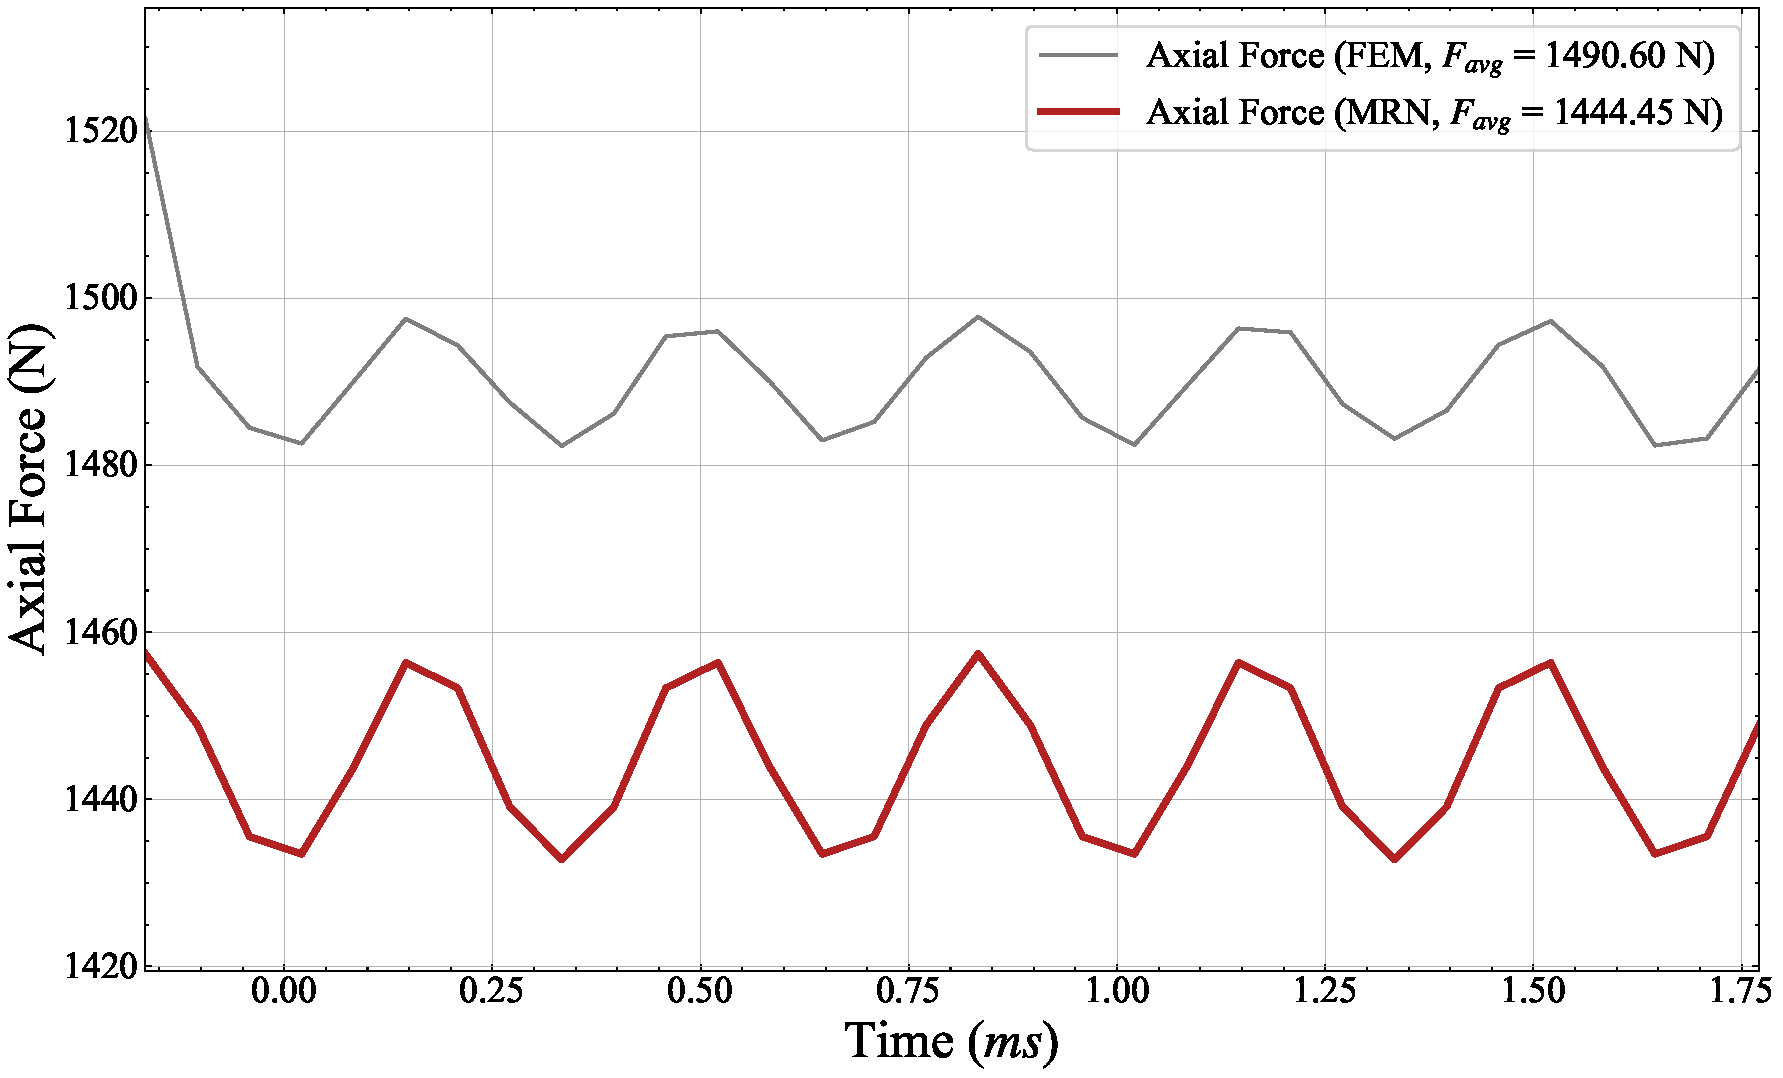
\includegraphics[width=0.45\textwidth]{figure/axial_force_no_load.png}
    \caption{Lực hút dọc trục không tải}
    \label{axial_force_no_load}
\end{figure}

\subsection{Load Verification}

Để đánh giá toàn diện năng lực tính toán của bộ giải 3D-MBGRN đề xuất trong điều kiện vận hành thực tế, quá trình kiểm chứng trạng thái có tải (On-Load Verification) được thực hiện tại dòng điện kích từ định mức $10.0\text{ A}$ (RMS) và góc tiến dòng bằng $0.0^\circ$. Khác với trạng thái hở mạch thuần túy, phản ứng phần ứng (armature reaction) sinh ra bởi dòng điện các pha stator tạo ra trường điện từ xoáy phức tạp, tương tác và làm méo dạng từ trường kích từ gốc của hệ thống nam châm vĩnh cửu, đồng thời tác động đến hiện tượng bão hòa từ tính cục bộ bên trong lõi thép lamination steel 1008.

Trước hết, phân bố mật độ từ thông tổng thể dưới tác động kích từ kép được biểu diễn thông qua bản đồ từ trường (B-map) tại Hình~\ref{bmap}. Kết quả đối chiếu đồ thị giữa phương pháp 3D-MBGRN đề xuất và mô hình 3D-FEM đối chứng thể hiện sự tương đồng khá rõ về quy luật phân bố tổng thể. Sự dịch chuyển của các vùng mật độ từ thông cực đại cục bộ do hiện tượng lệch trục từ trường dưới tải được bộ giải đề xuất thể hiện phù hợp, phản ánh tính đúng đắn của việc thiết lập hệ phương trình ma trận độ dẫn toàn cục phi tuyến.

\begin{figure}[H]
    \centering
    \includegraphics[width=0.48\textwidth]{figure/bmap.png}
    \caption{Comparison of magnetic flux density distributions between FEM and the proposed 3D-MBGRN solver under rated load condition: (a) 3D isometric view, (b) cross-sectional view at the mid-airgap plane with the highlighted airgap probing path, and (c) bottom surface view.}
    \label{bmap}
\end{figure}

Đặc tính không gian của mật độ từ thông khe hở không khí trạng thái có tải được trích xuất dọc theo cung tròn probe line tại bán kính trung bình như mô tả trong Hình~\ref{bmap}.b. Các kết quả về dạng sóng transient và phổ hài (spatial harmonics) tương ứng được trình bày chi tiết tại Hình~\ref{airgap_flux_density} và Hình~\ref{airgap_flux_density_harmonic}.

\begin{figure}[H]
    \centering
    \includegraphics[width=0.45\textwidth]{figure/airgap_flux_density_waveform.png}
    \caption{Mật độ từ thông khe hở không khí ở trạng thái có tải}
    \label{airgap_flux_density}
\end{figure} 

\begin{figure}[H]
    \centering
    \includegraphics[width=0.45\textwidth]{figure/airgap_flux_density_harmonics.png}
    \caption{Phân tích phổ harmonic của mật độ từ thông khe hở không khí trạng thái có tải}
    \label{airgap_flux_density_harmonic}
\end{figure}

% Airgap flux density

Dữ liệu định lượng trích xuất cho thấy thành phần dọc trục ($B_z$) vẫn đóng vai trò chủ đạo với biên độ đỉnh đạt $0.88\text{ T}$ ở 3D-MBGRN so với $0.81\text{ T}$ ở 3D-FEM (độ lệch $8.49\%$). Trị hiệu dụng (RMS) của thành phần $B_z$ đạt mức $0.63\text{ T}$ so với $0.62\text{ T}$ (độ lệch đối chiếu là $1.87\%$). Đối với phân tích phổ hài tại Hình~\ref{airgap_flux_density_harmonic}, thành phần hài bậc cơ bản (Harmonic Order \#1) của mật độ từ thông dọc trục đạt mức tương đồng cao với giá trị $0.8513\text{ T}$ (3D-MBGRN) so với $0.8465\text{ T}$ (3D-FEM), tương ứng độ lệch tương đối khoảng $0.57\%$. Các thành phần hài bậc cao như bậc 3 ($0.1925\text{ T}$ so với $0.1767\text{ T}$, độ lệch $8.91\%$), bậc 5 ($0.1007\text{ T}$ so với $0.0662\text{ T}$) và bậc 7 ($0.0203\text{ T}$ so với $0.0162\text{ T}$) phản ánh tính phi tuyến bão hòa của răng stator cũng được ghi nhận với mức độ bám sát nhất định.

Hình~\ref{flux_linkage} biểu diễn đặc tính transient theo vị trí góc quay cơ học của từ thông liên kết pha A ($\Psi_a$) dưới điều kiện tải định mức. Do tác động tổng hợp từ dòng điện phần ứng, biên độ đỉnh của từ thông tăng lên mức $0.06\text{ Wb}$ trên cả hai phương pháp với độ lệch biên độ đỉnh ghi nhận ở mức $2.74\%$. Trị hiệu dụng RMS của từ thông đạt $0.04\text{ Wb}$ (độ lệch $2.83\%$). Sự tương đồng về mặt pha và dạng sóng của đại lượng tích phân toàn cục này thể hiện khả năng tính toán transient của bộ giải đề xuất.

\begin{figure}[H]
    \centering
    \includegraphics[width=0.45\textwidth]{figure/flux_linkage_waveform.png}
    \caption{Từ thông liên kết pha A ở trạng thái có tải}
    \label{flux_linkage}
\end{figure}

Do sức phản điện động có tải ($e$) phụ thuộc vi phân trực tiếp vào tốc độ biến thiên theo thời gian của từ thông liên kết, đại lượng này phản ánh tiêu chuẩn kiểm chứng độ chính xác động học của trường điện từ phi tuyến dưới tải. Hình~\ref{back_emf} trình bày sự đối chiếu dạng sóng transient của sức phản điện động pha A ($e_a$) ở tốc độ định mức $3000\text{ rpm}$.

\begin{figure}[H]
    \centering
    \includegraphics[width=0.45\textwidth]{figure/back_emf_waveform.png}
    \caption{Sức phản điện động pha A ở trạng thái có tải}
    \label{back_emf}
\end{figure}

Kết quả đồ thị cho thấy biểu đồ của bộ giải đề xuất bám sát mô hình đối chứng. Cụ thể, biên độ đỉnh của sức phản điện động tính toán bởi phương pháp 3D-MBGRN đạt $177.12\text{ V}$, so với giá trị $182.86\text{ V}$ thu được từ mô hình 3D-FEM với độ lệch đỉnh là $3.14\%$. Trị hiệu dụng (RMS) của hai phương pháp lần lượt đạt $122.97\text{ V}$ và $126.55\text{ V}$ (độ lệch $2.83\%$). Trên phương diện hài không gian, biên độ sóng hài bậc 1 đạt $173.81\text{ V}$ so với $178.87\text{ V}$ (độ lệch $2.83\%$), trong khi các thành phần hài bậc cao như bậc 5 ($5.64\text{ V}$ so với $5.66\text{ V}$, độ lệch $0.33\%$) và bậc 7 ($1.18\text{ V}$ so với $1.15\text{ V}$, độ lệch $3.16\%$) cũng đạt độ tương đồng nhất định.

Đặc tính mô-men điện từ transient dưới tải ($T$) được thể hiện tại Hình~\ref{torque}. Kết quả tính toán cho thấy giá trị mô-men đầu ra trung bình (DC component) đạt mức $9.93\text{ Nm}$ đối với phương pháp 3D-MBGRN và $9.90\text{ Nm}$ đối với phương pháp 3D-FEM, tương ứng với độ lệch tích phân toàn cục là $0.30\%$. Giá trị mô-men này đáp ứng yêu cầu kiểm chứng công suất đầu ra định mức của động cơ đạt xấp xỉ hơn $3.1\text{ kW}$ ($3120.76\text{ W}$ so với $3111.54\text{ W}$). Độ đập mạch mô-men (Torque Ripple Ratio) trích xuất từ mô hình mạng từ trở đạt giá trị $15.77\%$ so với mức $11.46\%$ của mô hình phần tử hữu hạn. Độ lệch biên độ đập mạch đỉnh-đỉnh này ($0.78\text{ Nm}$ so với $0.57\text{ Nm}$) xuất phát từ ảnh hưởng của hiệu ứng bậc thang (staircase effect) do việc rời rạc hóa lưới cố định cấu trúc trụ, tuy nhiên sự chênh lệch tuyệt đối này là nhỏ trong các bài toán thiết kế tối ưu hóa.

\begin{figure}[H]
    \centering
    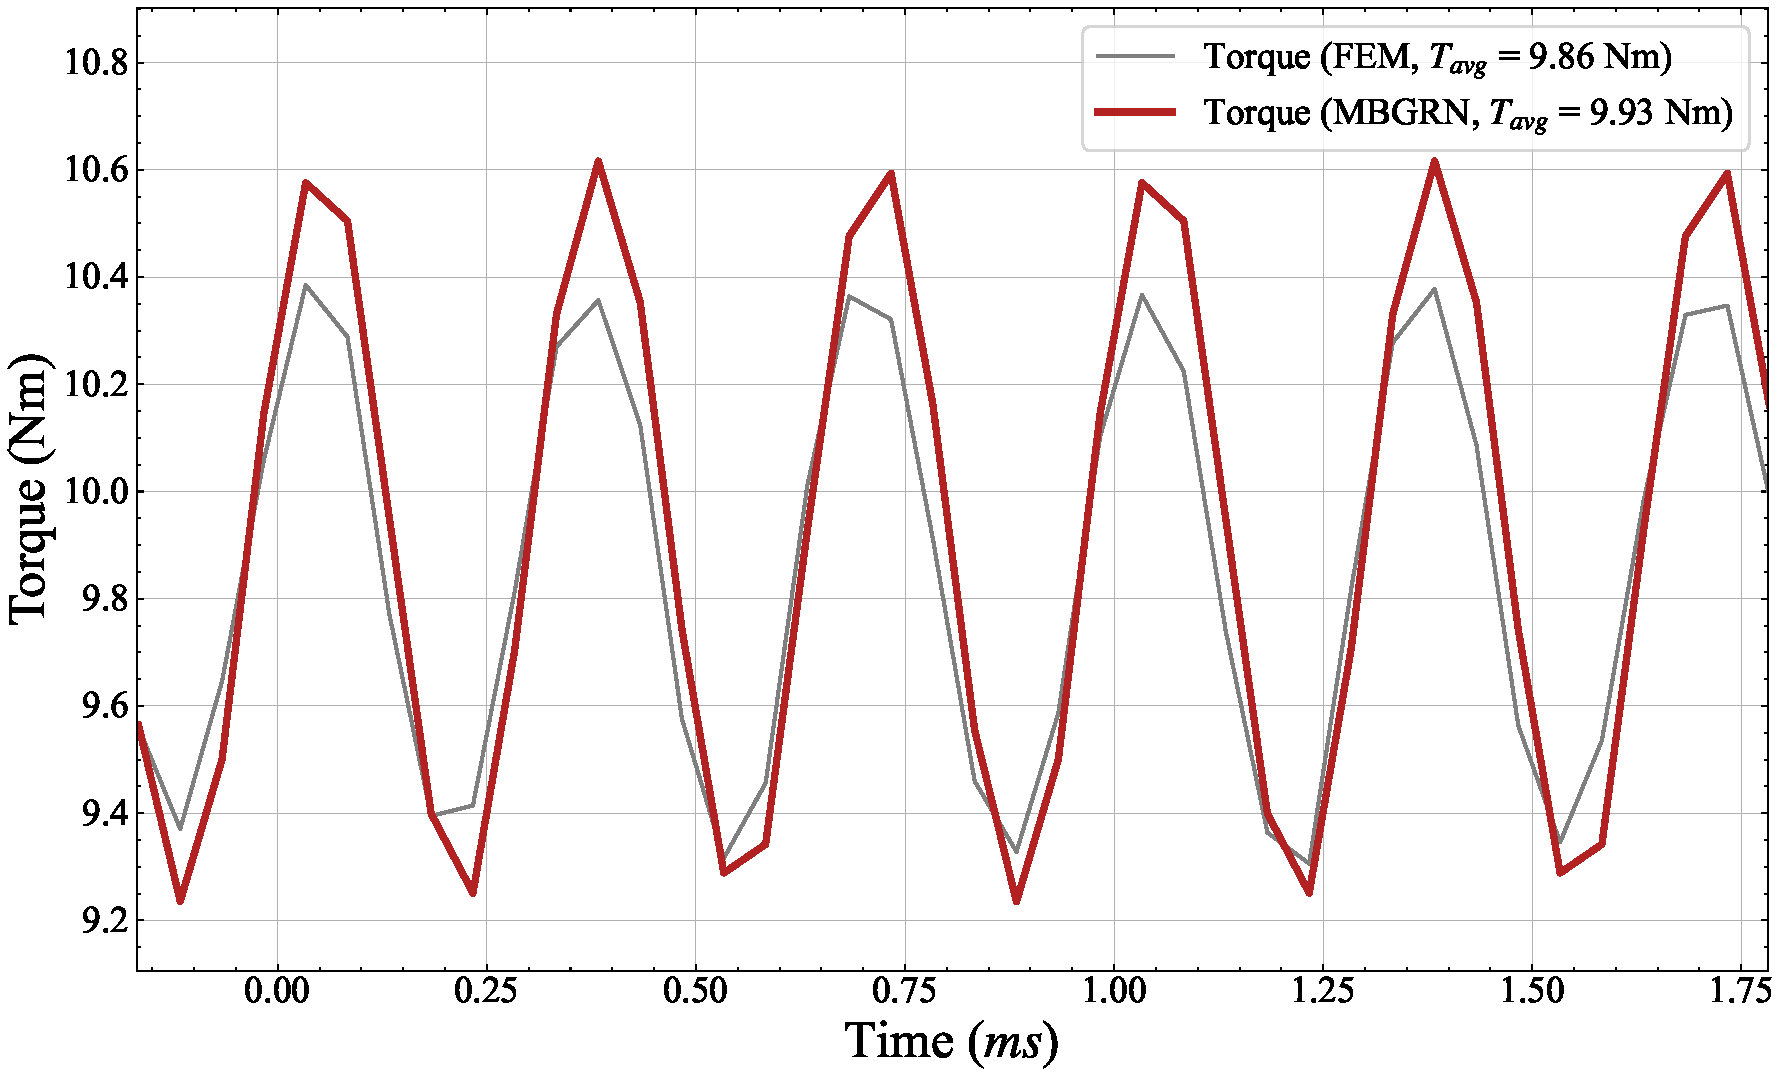
\includegraphics[width=0.45\textwidth]{figure/torque.png}
    \caption{Mô-men điện từ transient ở trạng thái có tải định mức}
    \label{torque}
\end{figure}

Đối với dòng máy điện hướng trục, lực hút dọc trục ($F_z$) tác dụng lên trục cơ khí dưới trạng thái tải là tham số quan trọng phục vụ việc tính toán độ bền cơ học và lựa chọn ổ đỡ hệ thống. Hình~\ref{axial_force} biểu diễn đặc tính biến thiên theo vị trí góc quay của lực dọc trục có tải. Dưới tác động của phản ứng phần ứng, giá trị lực tĩnh trung bình tổng thể ghi nhận ở mức $1453.01\text{ N}$ (3D-MBGRN) và $1499.50\text{ N}$ (3D-FEM), duy trì độ lệch bám sát ở mức $3.10\%$. Giá trị hiệu dụng RMS tương ứng của lực đạt $1453.05\text{ N}$ so với $1499.52\text{ N}$ (độ lệch $3.10\%$). Mặc dù có sự chênh lệch về biên độ dao động transient đỉnh-đỉnh ($14.20\text{ N}$ so với $20.29\text{ N}$), biên độ dao động này chiếm tỷ lệ nhỏ (chưa tới $1.5\%$) so với tổng lực từ tĩnh xấp xỉ $1500\text{ N}$, cho thấy khả năng đáp ứng của mô hình đề xuất khi dự báo tải trọng cơ khí.

\begin{figure}[H]
    \centering
    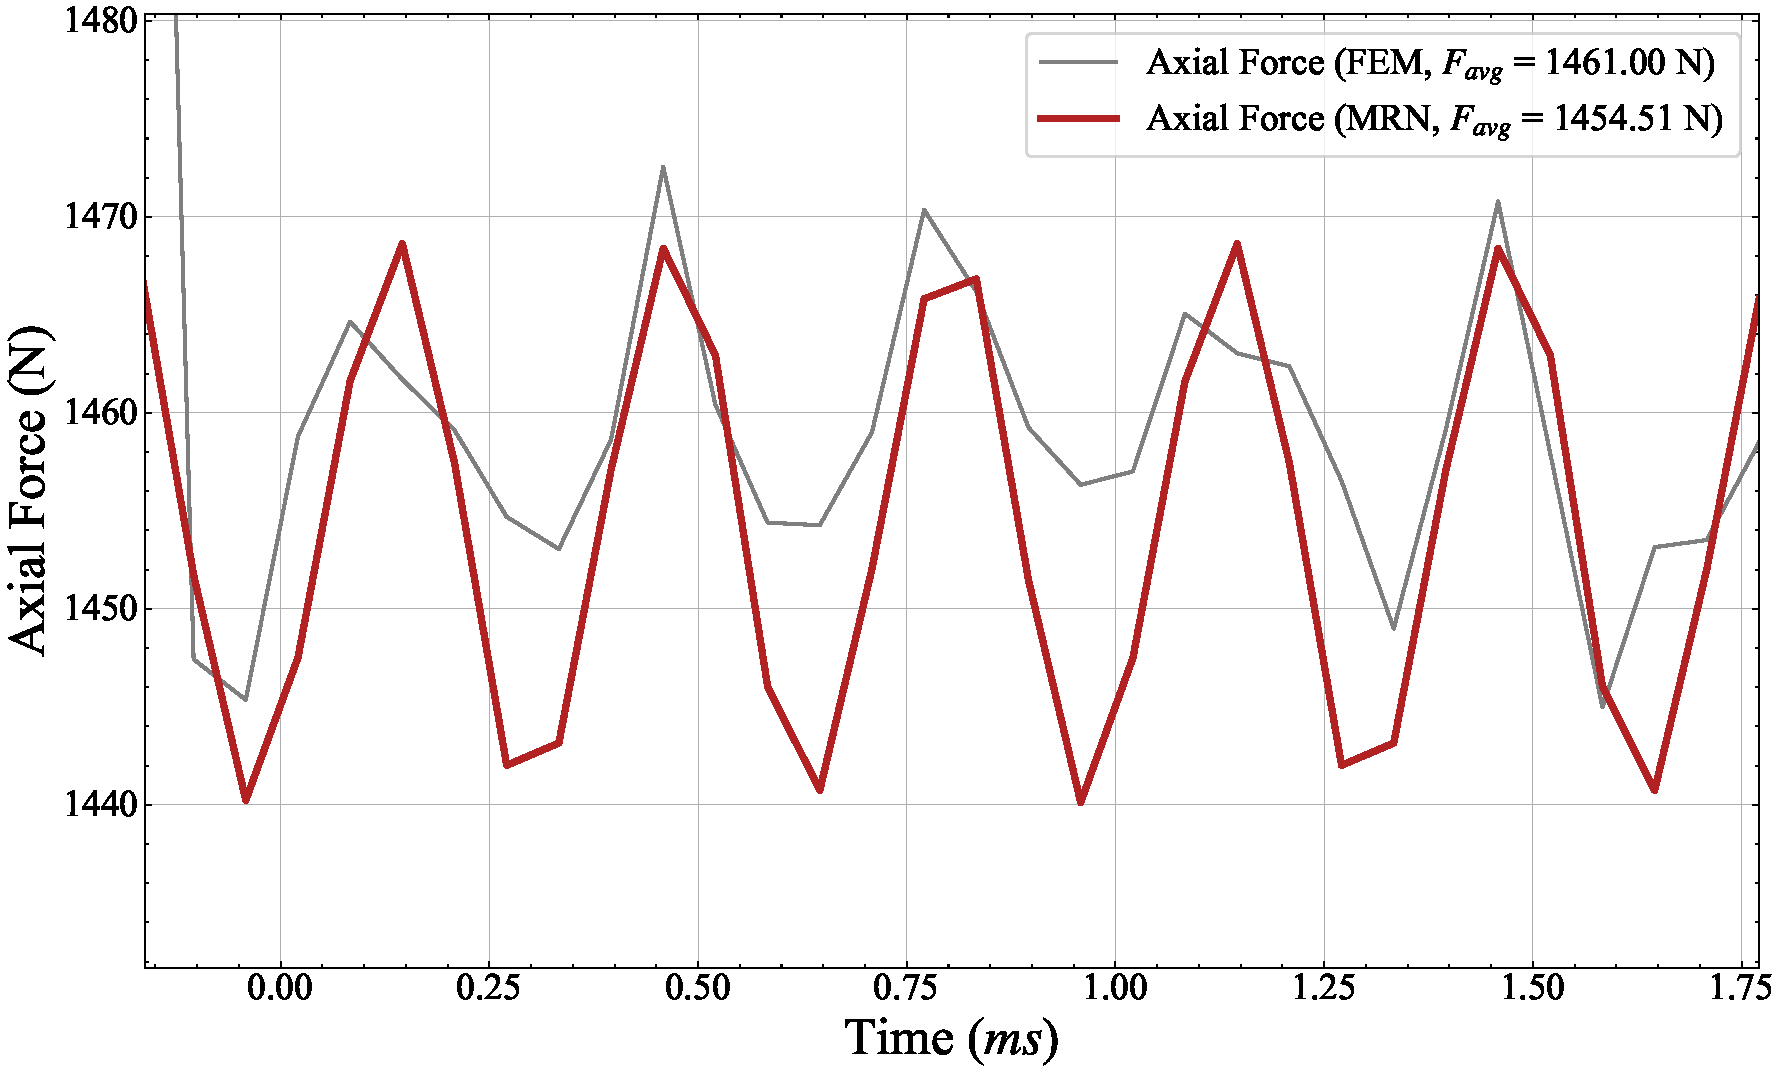
\includegraphics[width=0.45\textwidth]{figure/axial_force.png}
    \caption{Lực hút dọc trục transient ở trạng thái có tải}
    \label{axial_force}
\end{figure}

Cuối cùng, đặc tính biến thiên của công suất cơ học đầu ra theo sự thay đổi của biên độ dòng điện kích từ stator trong dải từ $0.0\text{ A}$ đến $20.0\text{ A}$ được biểu diễn tại Hình~\ref{current_power}. Kết quả đối chiếu cho thấy công suất cơ học tăng gần như tuyến tính theo biên độ dòng điện và ghi nhận sự tương đồng cao giữa hai phương pháp tính toán xuyên suốt toàn bộ dải khảo sát. Tại điểm làm việc với dòng điện kích từ định mức $10.0\text{ A}$, công suất cơ học đầu ra tính toán bởi bộ giải 3D-MBGRN đạt $3120.76\text{ W}$, bám sát giá trị $3111.54\text{ W}$ thu được từ mô hình 3D-FEM đối chứng với độ lệch tương đối chỉ $0.30\%$. Ngay cả ở dải dòng điện cao ($15.0\text{ A} \div 20.0\text{ A}$) nơi hiện tượng bão hòa từ tính phi tuyến xuất hiện rõ rệt hơn, đường đặc tính công suất từ bộ giải 3D-MBGRN vẫn thể hiện sự tương đồng phù hợp với 3D-FEM, cho thấy khả năng ứng dụng hiệu quả của phương pháp mạng từ trở 3D trong các bài toán thiết kế tối ưu hóa.

\begin{figure}[H]
    \centering
    \includegraphics[width=0.45\textwidth]{figure/current_power.png}
    \caption{Đặc tính công suất đầu ra tại các biên độ dòng điện kích từ khác nhau}
    \label{current_power}
\end{figure}